\documentclass{beamer}
\usetheme{Warsaw}

\title{Veiligheid en privacy}
\subtitle{Meer dan alleen maar encryptie}
\author{Kristof Provost}
\date{08 November 2014}
\subject{IEEE802.11}

\begin{document}
  \frame{\titlepage}

  \begin{frame}
    \frametitle{Over mij}
    \begin{itemize}
      \item Kristof Provost
      \item Freelance embedded software mens
      \item Huidig project: Wifi dingen bij SoftAtHome
        \pause
      \item (Niet te koop)
        \pause
      \item (Wel te huur)
        \pause
      \item (Redelijke prijzen!)
    \end{itemize}
  \end{frame}

  \begin{frame}
    \frametitle{Wifi: snel uitgelegd}
    You see, wire telegraph is a kind of a very, very long cat.  You pull his
    tail in New York and his head is meowing in Los Angeles.  Do you understand
    this? And radio operates exactly the same way: you send signals here, they
    receive them there.  The only difference is that there is no cat.
  \end{frame}

  \begin{frame}
    \frametitle{Associaties / netwerken ontdekken}

    \begin{itemize}
      \item Hoe verbindt een client met een wifi netwerk?
        \pause
      \item Wacht, hoe vindt een client een wifi netwerk?
        \pause
      \item Beacon frames!
        \pause
      \item en Probe Requests
    \end{itemize}
  \end{frame}

  \begin{frame}
    \frametitle{Een associatie}
    \framesubtitle{Voor WPA/WPA2}

    \begin{enumerate}
      \item Scan door kanalen
        \pause
      \item Vindt Beacon Frames
        \pause
      \item Stuur een Probe Request
        \pause
      \item Ontvang een Probe Response
        \pause
      \item Authentication Request/Response
      \item Association Request/Response
        \pause
      \item EAP / 802.1x key exchange
    \end{enumerate}
  \end{frame}

  \begin{frame}
    \frametitle{Beacon Frames}
    \begin{itemize}
      \item Uitgezonden door AP (typisch elke 100ms)
      \item "Hier is een acces point"
      \item Bevat:
        \begin{itemize}
          \item SSID
          \item Land code
          \item Informatie over versleuteling
          \item Traffic Indication Map (voor stations in power save mode)
          \item QoS informatie (WMM/WME)
          \item ...
        \end{itemize}
    \end{itemize}
  \end{frame}

  \begin{frame}
    \frametitle{Probe Request/Response}
    \begin{itemize}
      \item (Request) Uitgezonden door een station
      \item "Vertel eens wat meer over jezelf"
      \item Bevat:
        \begin{itemize}
          \item Veel van de informatie uit de beacon frames
          \item WPS (Wifi Simple Configuration) informatie
          \item ...
        \end{itemize}
    \end{itemize}
  \end{frame}

  \begin{frame}
    \frametitle{Wat is nu het probleem?}

    \begin{itemize}
      \item Verborgen netwerken
      \item Sturen geen SSID in hun Beacon Frames
      \item Dus, stations 'zoeken' er naar door Probe Requests te sturen
        \pause
      \item Altijd (als ze niet op een ander netwerk zitten)
      \item Overal
        \pause
      \item Ook voor niet verborgen netwerken (want die kunnen ondertussen verborgen zijn)
    \end{itemize}
  \end{frame}

  \begin{frame}
    \frametitle{qprobemon}
    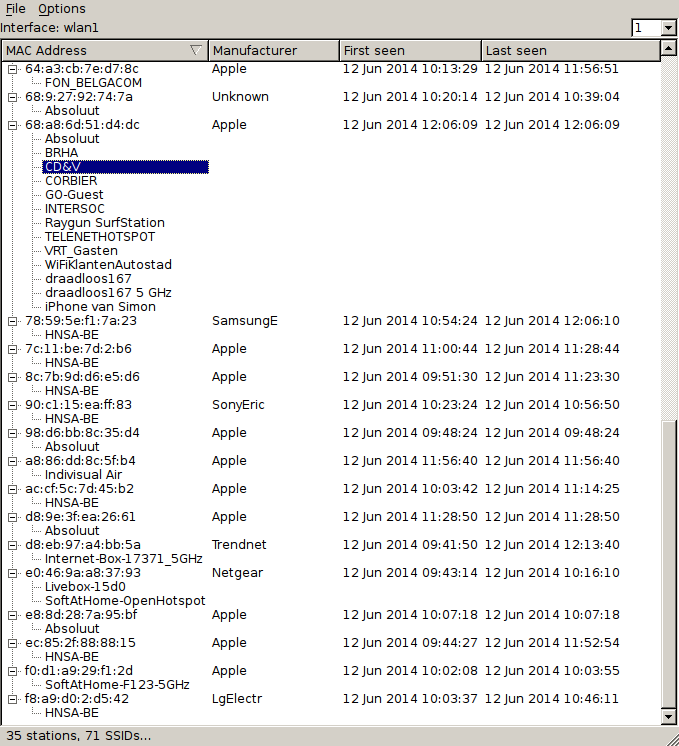
\includegraphics[keepaspectratio,width=\textwidth]{qprobemon-scary.png}
  \end{frame}

  \begin{frame}
    \frametitle{qprobemon}
    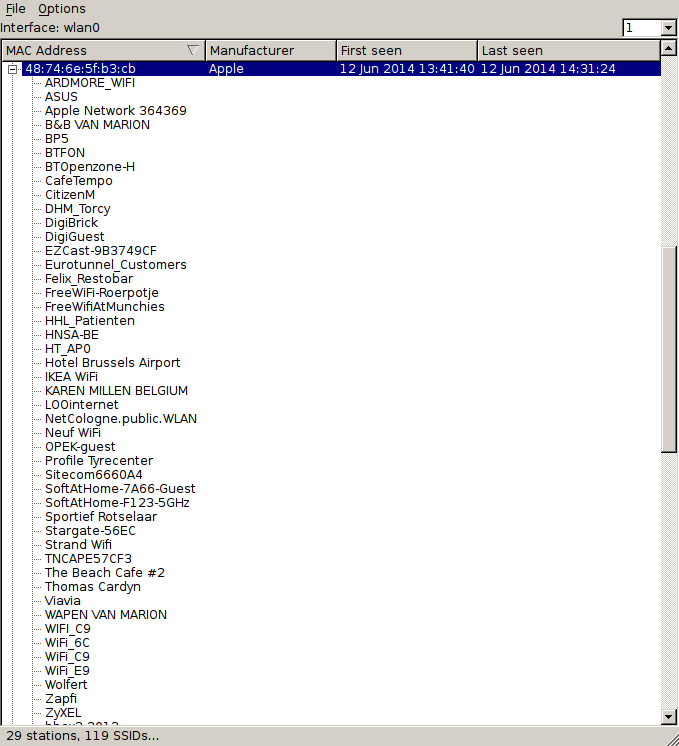
\includegraphics[keepaspectratio,width=\textwidth]{qprobemon-scary2.png}
  \end{frame}

  \begin{frame}
    \frametitle{qprobemon}

    \begin{itemize}
      \item Qt app
      \item Plaatst wifi interface in monitor mode
      \item Verzamelt Probe Requests
      \item Volledig passief (onmogelijk te detecteren)
      \item Code op GitHub
    \end{itemize}
  \end{frame}

  \begin{frame}
    \frametitle{Oplossingen?}

    \begin{itemize}
      \item Apple iOS 8 gebruikt willekeurige MAC addressen voor Probe Requests
        \begin{itemize}
          \item MAAR niet altijd
          \item zie http://blog.airtightnetworks.com/ios8-mac-randomgate/
        \end{itemize}
      \item Stop gewoon met Probe Requests te sturen
        \begin{itemize}
          \item Geen verborgen netwerken meer
          \item verborgen netwerken helpen toch niets
        \end{itemize}
    \end{itemize}
  \end{frame}

  \begin{frame}
    \frametitle{Einde}
    \begin{center}
      \Huge Vragen?
    \end{center}
    \begin{center}
      \small Mogelijk zelfs antwoorden!
    \end{center}
  \end{frame}

  \begin{frame}
    \frametitle{Referenties}
    \begin{itemize}
        \item Presentatie: \url{http://github.com/kprovost/wifi_privacy}
        \item Code: \url{https://github.com/kprovost/qprobemon}
        \item "Ik wil je geld geven:" \url{http://www.codepro.be}
    \end{itemize}
  \end{frame}
\end{document}
